\section{Lecture 15}
\subsection{Lecture Notes - Rotating Frame Clickers}
Which of the following motion leads to fictituous forces?
\begin{enumerate}[1.]
    \item The frame moves at a constant velocity with respect to an inertial reference frame.
    \item The frame rotates at a constant angular velocity with respect to an inertial reference frame.
    \item The frame moves at a constant acceleration with respect to an inertial reference frame.
    \item The frame rotates at a constant angular acceleration with respect to an inertial reference frame.
\end{enumerate}
\begin{s}
Three of these frames have fictituous forces (1 does not, its inertial). 2. We saw last day, 3/4 lead to fictituous forces as we will see today!
\end{s}
\noindent The coriolis and centrifugal "forces" are
$$
\begin{array}{l}
\mathbf{F}_{\text {coriolis }}=-2 \mathrm{~m} \boldsymbol{\Omega} \times \mathbf{v} \\
\mathbf{F}_{\text {centifitigal }}=-\mathrm{m} \boldsymbol{\Omega} \times(\boldsymbol{\Omega} \times \mathbf{r})
\end{array}
$$
Which force is more important in the limit of slow velocity (in the rotating frame)?
\begin{s}
In the limit of slow velocity, the centrifugal force (independent of velocity) dominates (the Coriolois force is linear in velocity).
\end{s}
A disk drive typically rotates at $3600$rpm, or $360$ radians per second. For a dust particle at radius $r = 5$cm, how fast must the particle be moving (in the rotating frame) for the Coriolis and the centrifugal forces to have approximately equal magnitude?
\begin{s}
Equating the two expressions and solving for $\abs{\v{v}}$, we find that $\abs{\v{v}} = 900$cm/s.
\end{s}
\noindent A hockey puck slides from the center towards the edge of a frictionless, rotating merry-go-round. The merry-go-round has angular velocity $\Omega$ and rotates CCW when viewed from above. In the rotating frame, the initial velocity is in the positive y direction. In the \textbf{inertial} frame, which way does the path of the puck bend?
\begin{center}
    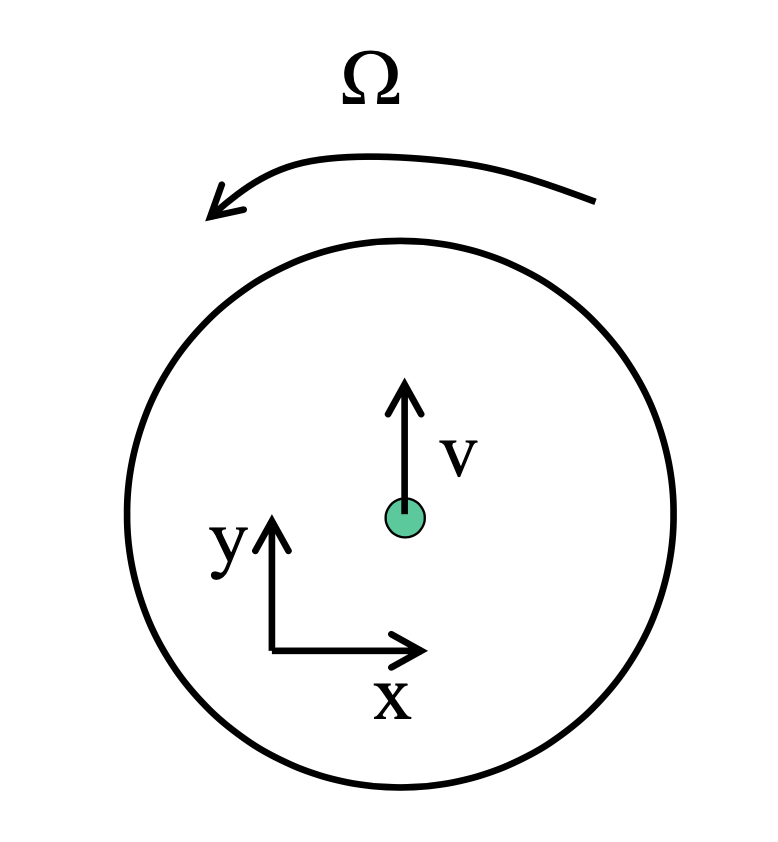
\includegraphics[scale=0.3]{Lecture-15/w15-img3.png}
\end{center}
\begin{s}
The path of the puck does not bend in the inertial frame; it retains a straight trajectory (there is no force acting on it!)
\end{s}
\noindent In the rotating frame, which way does the path of the puck bend?
\begin{s}
Applying the RHR, we see that the path curves to the right when viewed from above (towards positive $x$).
\end{s}